\section{Introduction}
\label{sec:intro}

Key/value stores remain a fundamental building block of modern
scale-out service architectures.  Recent trends in primary storage
technologies, however, are pushing operators to consider ever-more
disaggregated designs for their in-memory storage systems.
Concretely, increases in CPU core counts coupled with stagnating DRAM
density has led to an increased interest in remote memory tiers, where
some portion of memory is connected to the server over a network.
Moreover, once disaggregated, memory can be pooled to achieve greater
cost and power efficiencies.  The challenge facing fully disaggregated
memory pools, however, is managing concurrent updates in the face of
client failures and high access latencies.
%---e.g., 20$\times$ in the case of Ethernet-based RDMA.

While cache-coherent technologies like CXL are beginning to
become available, RDMA remains the commodity option for
large-scale in-memory key/value stores.
%% % made DRAM a scarce resource. In response data center
%architects have % proposed resource disaggregation to
%improve resource utilization, % scalability and efficiency
%as well as increase per-core access to % memory.
%Disaggregation calls for the partitioning of a servers %
%resources into distinct pools (compute, memory, storage, %
%accelerators), which are interconnected by a high speed
%network.  In a % fully disaggregated model distinct servers
%house resources such as % memory servers which contain only
%memory, and no collocated CPU for % processing.  DRAM
%capacity is scaling at an ever decreasing rate. As such the
%demand in data centers for high efficiency memory systems
%grows every year to improve memory utilization and sharing.
%Memory disaggregation i.e separating compute and memory
%into large pools is a promising approach to increase a
%CPU's per core memory access beyond what is available in a
%single machine while simultaneously decreasing per machine
%memory stranding.
%
%% Full disaggregation is challenging as it requires new
%system % designs to cope with the additional network
%latency.  For % example accessing intra-rack remote DRAM
%has a 20x (50ns to % 1us) overhead in relation to local
%memory. Cores sharing % remote memory must suffer a
%proportionally high cost for % synchronization when sharing
%pools of memory.  Many prior disaggregated systems have
%eschewed sharing for static partitioning to avoid the high
%overheads~\cite{ reigons,blade-server,legoos}.
Many prior RDMA-based systems opt for a partially
disaggregated model, in which a CPU core is collocated with
remote memory to provide the needed
serialization~\cite{erpc,herd,pilaf,cell,clover,sherman}.
%%  ~\cite{clover}. These designs are conceptually % close
%to prior work on RDMA key value stores which gain %
%performance benefits from having some operations use %
%one-sided RDMA verbs\footnote{one-sided verbs are %
%disaggregation compliant as they do not require a CPU on
%the % receiver side during operation} % %% % % While highly
%performant these approaches do not conform to % fully
%disaggregated designs.
%
%to remote memory are approximately 20x that of local DRAM
%(50ns to 1us) which severely increases the cost of
%synchronizing shared data structures among many CPU's
%across multiple machines. Traditional and partially
%disaggregated key-value serialize updates with a CPU
%collocated with
%memory~\cite{memcached,herd,erpc,pilaf,cell,clover}(\todo{check
%Sherman}). This approach does not meet the requirements of
%full disaggregation in which memory is a passive resource.
%In the fully disaggregated setting serialization is
%achieved entirely with a client based protocol. 
%
Fully disaggregated systems rely upon one-sided RDMA atomic
operations (e.g., compare-and-swap) to resolve data
races~\cite{rolex,fusee,race} which constrains their design.
%suffer from the limited scope of such operations.
Specifically, RDMA atomic operations can act upon 64 contiguous bits
of memory at a time at most, leading to implementations that employ
multi-stage datastructures to support practical key and value sizes.

In general, existing systems rely upon a high-performance index
structure to localize key operations and maintain values separately,
necessitating multiple RDMA operations and network round trips even in
the absence of contention.  Moreover, given the dominance of
read-heavy workloads~\cite{rocks-db-workload,facebook-memcached}, most
systems eschew locks in favor of optimistic update approaches that can
lead to poor performance under contention.
%
%optimistically update the index with pointers to
%enable lock-less reads avoid locking overheads and failures with
%visible partial writes.  Unfortunately, optimistic approaches can
%perform worse under high contention and demand indirect reads, leading
%to an awkward trade space.
%
%% These approaches either use optimistic
%% concurrency, or assume that most clients are collocated and
%% can resolve their lock acquisitions in local memory.
%% Optimistic approaches using RDMA atomics are limited by the
%% width of the atomic instruction (64 bits for compare and
%% swap). 64 bits is often too small to encapsulate a full
%% key-value update. The result is that optimistic approaches
%% require more round trips to remote memory to complete their
%% operations. These approaches have dismissed lock based
%% approaches outright as the size of their critical sections
%% can bottleneck performance, and  the cost of acquiring and
%% releasing locks (at minimum two round trips) is often higher
%% than the optimistic approach (two or three round trips).
%
% %concurrent data structures round trips
% Concurrent data structure design for remote memory is hard.
% Access latency to remote memory is high so round trips per
% operation must be minimized to achieve efficiency.
% Serialization is particularly hard because there is no
% centralized serialization point to guard access to remote
% memory. RDMA NIC's provide atomic verbs such as
% compare-and-swap (CAS), but these are by no means a silver
% bullet.  Each atomic request takes a round trip from client
% to server to execute. In the best case lock/unlock requires
% two round trips, if multiple locks are required, or locks
% are contested the number of round trips increases.
%
% %CPU locking vs RDMA
% In traditional key-value stores (Memcached~\cite{memcached})
% the CPU coordinates table access for read, write, and lock
% instructions. In contrast RDMA based Key-value
% stores~\cite{herd,erpc,pilaf} use a mixture of one-sided (no
% CPU) and two-sided (CPU involved) verbs to alleviate the CPU
% bottleneck. Reads are typically one sided to bypass the CPU
% bottleneck~\cite{pilaf,cell} while writes are typically two
% sided so memory-side CPU can orchestrate serialized
% operations (e.g. locking) with main memory access latency
% (50-100ns).  These small access times keep critical sections
% small for CPU based locking, and dramatically increase them
% for one-sided RDMA based locking schemes~\cite{clover,
% Sherman}.
%
%RDMA and cuckoo hashing
In this work we design an index datastructure tailored for the
constraints of current RDMA hardware.  Specifically, we
facilitate lock-based updates by decreasing the number of round
trips required to acquire locks and perform mutating operations.

We introduce RCuckoo, a fully disaggregated key/value store based on
cuckoo hashing~\cite{cuckoo} that
%delivers high performance using
uses only one-sided RDMA operations.
%At its heart,
RCuckoo builds
around a \emph{dependent hashing} algorithm that makes spatial
locality a tunable parameter.
%
%Locality enables us
%to effectively predict the locks, and rows required to perform
%operations and to set multiple locks with a single atomic
%operation. We design and implement a fast fault tolerance algorithm
%which allows distributed clients to detect and repair failures in the
%table while still issuing millions of operations per second.
%
%%  The core insight of our work is
%% that round trips can be decreased by increasing locality in
%% the table and the size of reads.
%
% Dependent hashing increases the likelihood that
% a key's hash locations will be spatially near one another;
% if locations are close enough, a client can read them both
% with a single RDMA operation.  Of course, the increased
% locality leads to a higher degree of collisions, impacting
% the maximum number of elements which can be inserted into
% the table (i.e., fill factor).  We explore the trade space
% to find the best balance  between performance and fill
% factor. Using this locality we design a dense lock table
% which can fit into RDMA NIC device memory as it provides up
% to 3$\times$ higher performance for contested atomic access.
% Our locking protocol acquires and releases locks in bulk
% using the fewest round trips possible. We use Masked Compare
% and Swap to remove unnecessary contention from out lock
% table.
%
% Using locks rather than CAS to modify our index allows our
% index to support variable sized entries, and allows us to
% inline keys and values directly into the index. Inlining
% entries significantly reduces operation latency. We highly
% optimize inserts into our hash table. Locality between
% key-pairs improves insert locality enabling RCuckoo to both
% find valid cuckoo paths efficiently and acquire all locks for
% insertion in few round trips. We achieve this with a mixture
% of smart caching, searching, and a two stage cuckoo path
% finding algorithm. Finally locality improves reads by using
% single larger reads when key pairs are close, rather than
% multiple smaller reads.
%
% Inserting into a cuckoo hash table normally requires
% acquiring many locks randomly throughout the table,
% dependent hashing clusters lock acquisitions enabling many
% locks to be acquired in a single atomic request. Second, our
% algorithm uses speculative lock acquisition. Locks are
% acquired in bulk based on a local cache of the remote index.
% Once locks are held a second search on synchronized locked
% data is performed to ensure a correct insertion. Third we
% use locality to improve both read and search speeds. We find
% that using a single large read over two smaller reads
% improves throughput when key locations are known to be
% physically close.
%
% \sg{Sherman uses masked compare and swap as well as device
% memory, we might use it better but it's hard to claim a
% contribution here.}
%
%Prior work suggests many important real-world workloads are
%read-heavy, with most objects being small.
RCuckoo employs a set of
complimentary techniques that leverage this enhanced locality to deliver higher performance than any prior
disaggregated key/value store while gracefully handling client
failures:

\begin{itemize}
\item{\textbf{Deterministic lock-free reads.}  Cuckoo hashing ensures
  an entry is always located in one of two locations which can be
  read in parallel.}

\item{\textbf{Space-efficient locks} frequently allow clients to acquire necessary 
  locks in a single RDMA operation.}

\item{\textbf{Client-side caching} enables accurate cuckoo-path
  speculation to improve insert performance.}

\item{\textbf{Leased lock acquisitions} allow clients to detect
  and recover from client failures using timeouts.}
\end{itemize}

%% message round-trips for both reads and writes,
%% improving performance for small-object reads and significantly
%% improving writes.


\begin{figure*}[t]
    \centering
    \begin{subfigure}{0.3\linewidth}
        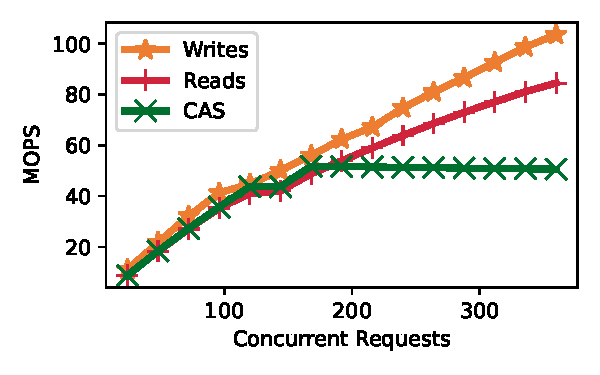
\includegraphics[width=0.99\linewidth]{fig/rdma_concur.pdf}
        % \label{fig:optimistic_failures}
        % \caption{}
    \end{subfigure}
    \begin{subfigure}{0.3\linewidth}
        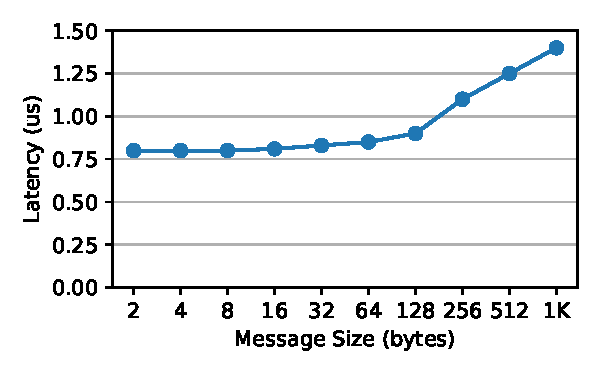
\includegraphics[width=0.99\linewidth]{fig/rdma_latency.pdf}
        % \label{fig:rdma_latency}
        % \caption{}
    \end{subfigure}
    \begin{subfigure}{0.3\linewidth}
        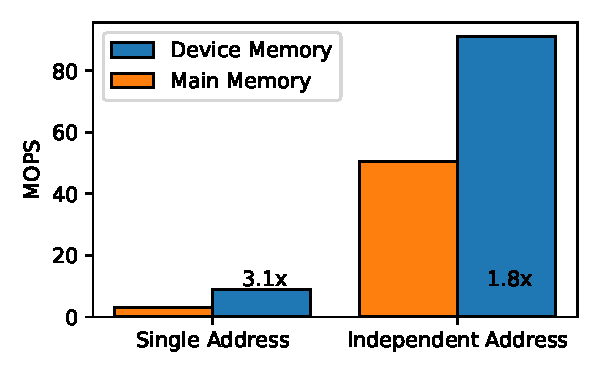
\includegraphics[width=0.99\linewidth]{fig/rdma_cas_throughput.pdf}
        % \label{fig:optimistic_failures}
        % \caption{}
    \end{subfigure}
    \vspace{-1em}
    \caption{Basic RDMA performance on our testbed.
    \textbf{(a)} (64-bit) operations per second;
    \textbf{(b)} operation latency as a function of message size~\cite{rdma-latency}; and
    \textbf{(c)} compare-and-swap performance on device and main memory.
    }
    \label{fig:rdma-benchmarks}
\vskip -1em
\end{figure*}

Combined with a datastructure design that facilitates aggressive
batching of RDMA operations, these techniques enable RCuckoo to limit
the number of round trips required for all table operations.  In the
common case, reads execute in one or two (for large values) round
trips, uncontested updates and deletes require two round trips, and
the median insert operation involves only two round trips---although
the expected number increases as the table fills.  On our testbed,
RCuckoo delivers comparable or higher performance on small values across the standard set  of YCSB benchmarks than all of the existing disaggregated
key/value stores we consider.  Concretely, with 320 clients RCuckoo
delivers up to a 2.5$\times$ throughput improvement on read-intensive
(YCSB-B) workloads and 0.9--7.1$\times$ the throughput on skewed
write-intensive (YCSB-A) workloads.  Moreover, RCuckoo's
performance remains high despite failure rates on the order of 100s of
clients per second.
